
% What is physical reservoir computing?
The RC model easily extends to the physical world by interpreting physical systems that exhibit nonlinear dynamics and memory effects as a reservoir substrate  \citep{nakajima_physical_2020}. 
In other words, this Physical Reservoir Computing (PRC) framework aims to exploit dynamics found in the natural world to perform computational tasks. 
% How is RC transferred to the real world?
\mbox{Figure \ref{fig:prc_examples}} shows a mapping of the RNN-based RC architecture to two physical applications from the literature and the plant RC case discussed in this thesis.
In the physical systems (\mbox{Figures \ref{fig:prc_examples}}b, c, and d), it is impossible to observe the complete state of the reservoir as in the RNN-based reservoir. 
Instead, the reservoir state is inferred from sensor data observing the dynamical system in real-time \citep{burms_reward-modulated_2015, nakajima_information_2015}.

\begin{figure}[t]
	\centering
    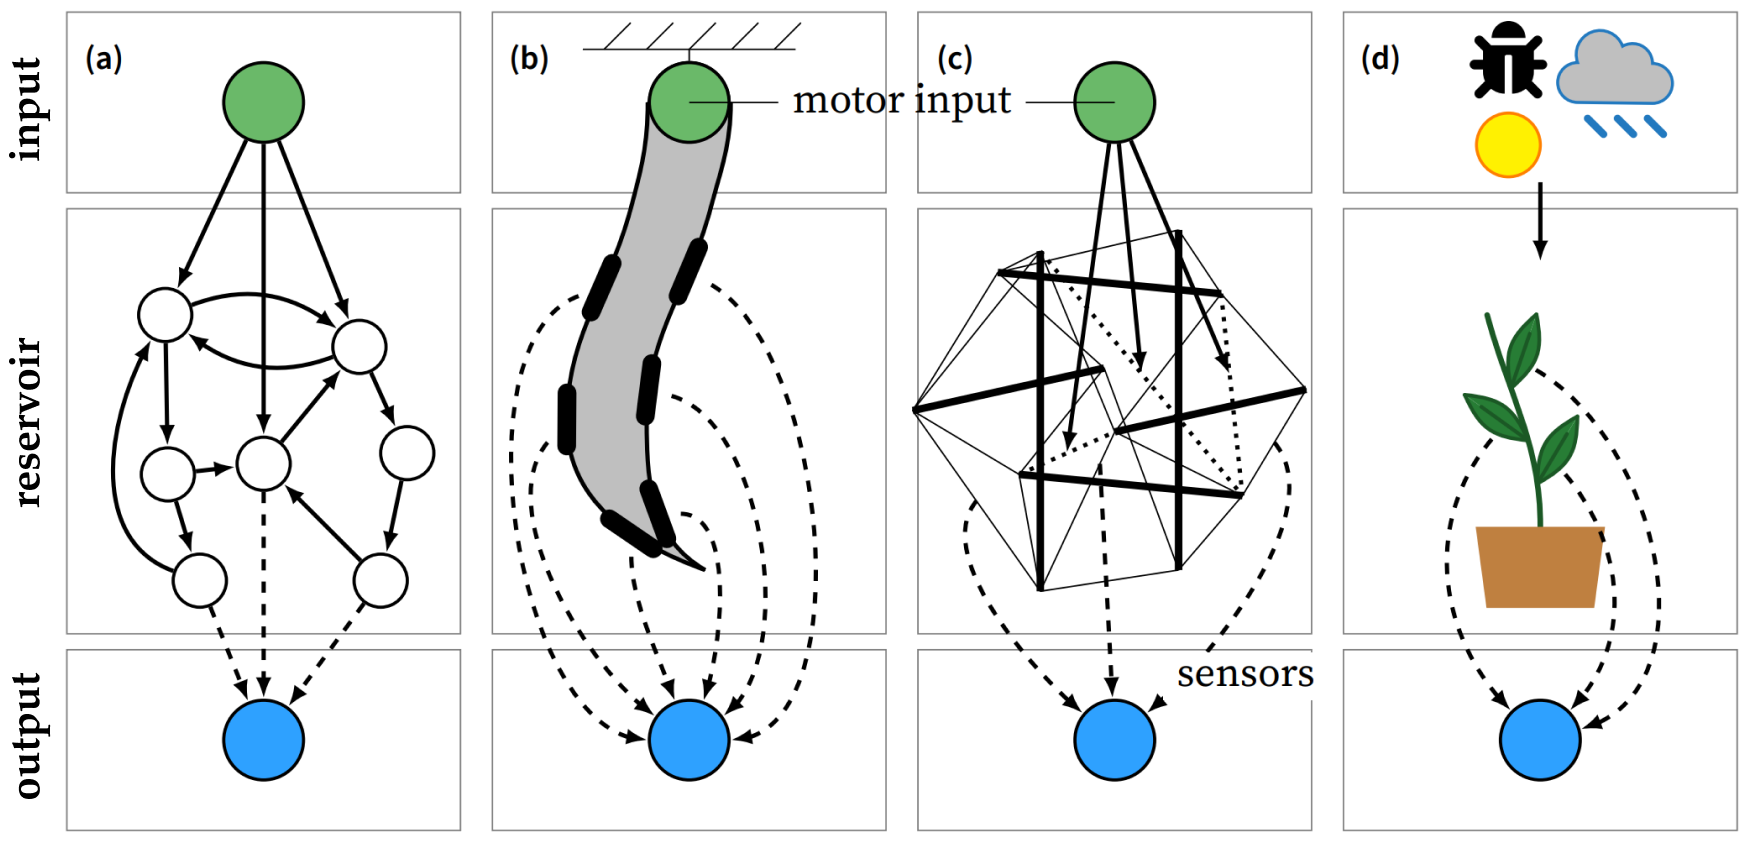
\includegraphics[width=0.9\textwidth]{img/prc-illustration.png}
    % \vspace{0.5cm}
    % \includegraphics[width=0.5\textwidth]{example-image}
	\caption[Illustration of different reservoir computing implementations, both theoretical and physical versions.]
	        {Illustration of different reservoir computing implementations, both theoretical and physical versions. 
	        Each of the subfigures depicts a different type of implementation: 
	            (a) RNN-based version; 
	            (b) soft body built of silicone \citep{nakajima_information_2015}; 
	            (c) compliant robot made of a tensegrity structure \citep{caluwaerts_locomotion_2013}; 
	            and (d) plant as reservoir.
    	 	Figure and caption reused from \citet{pieters_reservoir_2022} with permission from the author.}
	\label{fig:prc_examples}
\end{figure}

% What applications have been made with PRC?
PRC is a field of interdisciplinary research, implementing reservoirs using a large variety of materials \citep{tanaka_recent_2019}.
Examples of substrates being researched are analog electrical circuits \citep{soriano_minimal_2015, zhao_novel_2016}, FPGAs \citep{antonik_application_2018}, memristive circuits \citep{walter_neuromorphic_2015}, photonic circuits \citep{van_der_sande_advances_2017}, spintronics \citep{torrejon_neuromorphic_2017}, and soft body robotics \citep{caluwaerts_body_2011, caluwaerts_design_2014, nakajima_soft_2013}.
Biological reservoirs are closely investigated as well, with a particular interest in neurobiology \citep{hafizovic_cmos-based_2007, hinaut_real-time_2013} and ecological dynamics \citep{jones_is_2007, didovyk_distributed_2015,ushio_computational_2021}. 
Most recently, \citet{pieters_plants_2021} demonstrated promising results in the use of \textit{in vivo} plants as reservoir substrate.


% What is the goal of PRC research?
A common misconception about PRC research is that the goal is to achieve general-purpose computation with unconventional reservoirs. 
However, the aim is not to outperform silicon computers at carrying out generic calculations. 
Instead, in most cases, the goal is to bypass the need for precise modeling of a physical system by observing how the system responds to inputs rather than attempting to predict how the inputs influence the state of the system \citep{nakajima_physical_2020}.
This method is particularly applicable in real-time control scenarios such as robotics, where real-time integration of sensor data is more feasible than power-hungry physics simulations (see e.g.\ \cite{caluwaerts_design_2014, burms_reward-modulated_2015}), 
or for the prediction of chaotic systems where powerful computers are not able to predict the system better than low-powered reservoir models \citep{gauthier_next_2021}.


\subsection{Generalized Mathematical Model} \label{section:rc-general}

The mathematical model of the Echo State Network (section \ref{subsection:esn}) can be generalized to describe any reservoir computer, physical or otherwise \citep{nakajima_physical_2020}. 
Doing so will be helpful to determine what defines the RC system's computational capacity in the following sections. 
This section establishes a mathematical vocabulary for describing any PRC model in discrete-time notation.

The reservoir update function can be described as a function $f(\cdot, \cdot)$ that maps the previous reservoir state and the current input to a new reservoir state,
 
\begin{equation} \label{prc:update}
    \mathbf{x}[t] = f\left(\mathbf{x}[t-1], \mathbf{u}[t]\right) 
\end{equation}

where $\mathbf{x}$ describes the entire reservoir state at step $t$ and $\mathbf{u}$ represents all external factors that influence the dynamics of the reservoir substrate. 
Assuming the reservoir dynamics result in emergent memory effects, it is possible to reformulate the reservoir state $\mathbf{x}$ as a function of the past inputs it has seen:

\begin{equation} \label{prc:echo_input_function}
    \mathbf{x}[t] = \phi(\mathbf{u}[t], \mathbf{u}[t-1], \mathbf{u}[t-2], \dots)
\end{equation}

This function $\phi$ is called the input echo function and is a key characteristic of each particular reservoir substrate. The target task is defined as any arbitrary function $T$ of the past time steps, thus requiring memory to solve:

\begin{equation} \label{prc:target}
    \mathbf{y}[t] = T(\mathbf{u}[t], \mathbf{u}[t-1], \mathbf{u}[t-2], \dots)
\end{equation}

Finally, the linear readout function $\psi$ is described as a learned approximation of $T$, based on the reservoir state:

\begin{align} 
    \psi(\mathbf{x}[t]) &= \psi \left( \phi(\mathbf{u}[t], \mathbf{u}[t-1], \mathbf{u}[t-2], \dots) \right) \label{prc:readout} \\
    &\approx T(\mathbf{u}[t], \mathbf{u}[t-1], \mathbf{u}[t-2], \dots) = \mathbf{y}[t] \nonumber
\end{align}

It is important to note that the input echo function $\phi$ is surjective for virtually all reservoirs. 
In other words, a unique sequence of inputs does not necessarily result in a sequence of unique reservoir states. 
Not only is this natural, as no reservoir can have infinite memory of past events, Section \ref{section:esp} shows that this summarizing property of $\phi$ is vital to derive any meaningful computation from reservoir computers.